\documentclass[a4paper,11pt]{article}
%BIBLIOTECAS==================================================================================%
\usepackage[latin1]{inputenc}
\usepackage[brazil]{babel}
\usepackage{fancyhdr}
\usepackage{amsmath}
\usepackage{amsfonts}
\usepackage{amssymb}
\usepackage{graphicx} %para inserir figuras
\usepackage{subfigure} %para inserir subfiguras
\usepackage{url} %para links
\usepackage[normalem]{ulem}
\usepackage{epstopdf}
\usepackage{titlesec}
\usepackage{setspace}
\usepackage{cite}
\usepackage{indentfirst} %primeiro par�grafo
\usepackage[font=small,format=plain,labelfont=bf,up,up]{caption} %customiza legendas
\usepackage[a4paper,left=3cm,bottom=2cm,right=2cm,top=3cm]{geometry} %para definir as margens
\usepackage{listings} %para formatar c�digo-fonte
\lstset{numbers=left, numberstyle=\tiny, stepnumber=1, numbersep=5pt,basicstyle=\scriptsize,frame=single} %para c�digos
\usepackage{float} %posicao das legendas
\usepackage{multicol} %subcolunas
\usepackage{enumitem} %itens
%=============================================================================================%
\setlength{\parindent}{25pt}
%\setlength{\parskip}{0ex}
\onehalfspacing
%=============================================================================================%
%\titleformat{\part}[frame]{\normalfont}{\filright\footnotesize\enspace\thepart\enspace}{1em}{\Large\bfseries\filcenter}
%\titleformat{\section}[block]{\bfseries}{\thesection.}{1em}{\MakeUppercase}
%\titleformat{\subsection}[block]{\normalfont}{\thesubsection.}{1em}{\MakeUppercase}
%\titleformat{\subsubsection}[block]{\normalfont}{\thesubsubsection.}{1em}{}
\renewcommand{\lstlistingname}{Script}
\DeclareCaptionLabelSeparator{minus}{ - }
\captionsetup[FLOAT_TYPE]{labelformat=simple, labelsep=colon}
\captionsetup[figure]{labelsep=minus}
\captionsetup[table]{labelsep=minus}
\captionsetup[lstlisting]{labelsep=minus}
\floatstyle{plaintop}\restylefloat{table} %legenda das tabelas no topo
\addtolength{\belowcaptionskip}{-4pt} %espaco entre legendas
\addtolength{\abovecaptionskip}{-2pt}

%=============================================================================================%
\begin{document}
	\thispagestyle{empty}

\begin{figure}[t]
\centering

\includegraphics[scale=0.6]{Imagens/Logo.png}
\end{figure}

{\centering\linethickness{3pt}\line(1,0){455}}\\

\begin{large}
	\centering
	CENTRO DE TECNOLOGIA E URBANISMO\\
	DEPARTAMENTO DE ENGENHARIA EL�TRICA\\
	2ELE049 - Redes de Telecomunica��es\\[1.4in]
	\textbf{Experi�ncia 1: Desempenho de sistemas PAM}\\
	PROFESSOR: Jaime Laelson Jacob\\
	ALUNOS: David Krepsky\\
	Marco Aur�lio Hernandes Fortes\\
\end{large}

\begin{flushright}
\parbox{2.1in}
{
Relat�rio apresentado a disciplina de Redes de Telecomunica��es.\\
Experimentos(s) realizado(s) em: 13/10/2015.\\
Turma: 1012.\\[1.4in]
}
\end{flushright}

\begin{large}
	\begin{center}

	Londrina, \today \\
	\end{center}
\end{large}

{\centering\linethickness{3pt}\line(1,0){455}}

    \thispagestyle{empty}
\section*{Resumo}
Nesse relat�rio ser� analisado a simula��o de diversos sistemas digitais PAM, e ser� visto como comparar o desempenho dos diferentes circuitos, atrav�s da curva BERxSNR. E tamb�m se analisar� a simula��o de densidade espectral de pot�ncia dos sistemas sinc e cosseno levantado.
\newpage
	\thispagestyle{empty} 
\tableofcontents 
\pagebreak 
%\thispagestyle{empty} 
%\listoffigures 
%\listoftables 
%\pagebreak
	%\section{INTRODUÇÃO}
%\addtocounter{section}{1}
%\setcounter{page}{1}



%\newpage

	\section{OBJETIVOS}
%\begin{itemize}
%\item ...
%\end{itemize}
 Simular os diferentes sistemas PAM digitais usando formas de onda diferentes  e identificar a que apresenta o melhor desempenho (BERxSNR). Al�m disto, � necess�rio obter a simula��o da densidade espectral de pot�ncia dos sistemas sinc e cosseno levantado.




\newpage
	\section{REVIS�O DA LITERATURA}

\subsection{Sistemas Digitais}

Atualmente, a maior parte dos sistemas de comunica��o utilizam Modem digital. Porque este tem uma maior capacidade de canal,o desempenho de transmiss�o e recep��o � melhor, obtendo assim, uma menor BER. E quando utilizamos sinais digitais conseguimos um sinal sem ru�do adicionando um c�digo de corre��o de erro. E ainda obtemos uma maior efici�ncia de banda.

\subsection{Modula��o PAM}

A Modula��o de amplitude de impulso ou PAM � a transmiss�o de dados atrav�s da varia��o de amplitude dos n�veis de�tens�o�ou�pot�ncia� dos impulsos individuais numa sequ�ncia temporizada regular de impulsos el�tricos ou eletromagn�ticos.�O n�mero de poss�veis amplitudes de impulso pode ser infinita (no caso de PAM anal�gico), mas, geralmente, � uma pot�ncia de dois, de modo que o sinal de sa�da resultante pode ser digitalizado.�Em alguns sistemas de PAM, a amplitude de cada pulso � diretamente proporcional � amplitude de modula��o do sinal instant�neo no tempo o impulso ocorre.�Em outros sistemas PAM, a amplitude de cada pulso � inversamente proporcional � amplitude de modula��o do sinal instant�neo no tempo o impulso ocorre.�Em ainda outros sistemas, a intensidade de cada impulso depende alguma caracter�stica do sinal de modula��o diferente da sua for�a, tal como a sua instant�nea�frequ�ncia�ou�fase�.

\begin{figure}[H]
    \centering
    \caption{Sinal PAM retangular.}
    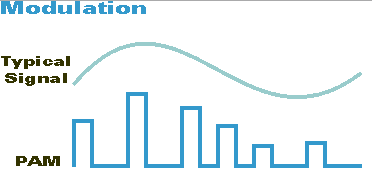
\includegraphics[scale=1]{Imagens/pam}
    \label{fig:Osci1}
\end{figure}

Em canais AWGN a detec��o coerente � �tima (min. BER) quando se utiliza matched filter ou filtro casado. O detector sincrono � �timo para canal AWGN requer custo de implementa��o mais elevado que a vers�o n�o-coerente.


A efici�ncia espectral do sinal PAM ou QAM com formata��o dos pulsos retangulares �:

\[
    \eta_{BW}^{MPSK_QAM}  = \frac{R}{B_T} = \frac{\mathrm{l}}{2} \, \bigg [ \frac{bits/s}{Hz} \bigg ]
\]

Onde   � o n�mero de pontos da constela��o de sinais.

Observe que a efici�ncia espectral aumenta � medida que o n�mero de pontos na constela��o cresce e o espectro do sinal em banda-base � reduzido (formata��o de pulso)

\newpage

	\section{METODOLOGIA EXPERIMENTAL}

\subsection{MATERIAIS}
Para o desenvolvimento das atividades propostas pelo experimento foi utilizado o software de simula��o OrCAD.

\subsection{M�TODOS}
A pr�tica no laborat�rio consistiu no desenho e simula��o deste circuito:
	\begin{figure}[H]
		\centering
		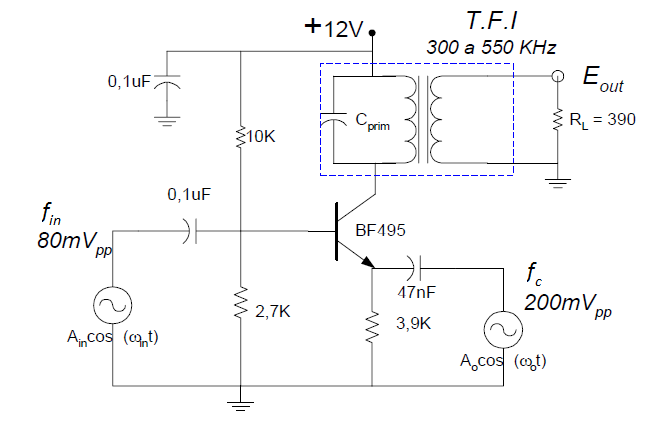
\includegraphics[scale=.6]{imagens/cir1.png}
		\caption{Circuito 1}
	\end{figure}

\begin{itemize}
	\item[$\bullet$] Atividade 1 - Determina��o do filtro
	\item[$\bullet$] Atividade 2 - Down-Converter e Up-Converter
	\item[$\bullet$] Atividade 3 - Uso de um amplificador seguidor de emissor
\end{itemize}

\subsubsection{Determina��o do filtro}
Foi necess�rio calcular os valores dos componentes que n�o est�o determinados: o indutor(transformador) e capacitor ligados ao coletor do transistor. Estes elementos formam um filtro passa faixas cuja frequ�ncia de oscila��o ditar� a frequ�ncia do sinal de sa�da. O transformador utilizado tem uma rela��o de espiras de 8:1, ou seja, o indutor do secund�rio deve ser 64 vezes menor do que o do prim�rio. 


	\section{RESULTADOS}
Nesta se��o ser�o discutidos os resultados obtidos pelos diversos experimentos.
\subsection{PAM retangular}

Para o circuito da Figura \ref{f1}, temos os gr�ficos apresentados pelos oscilosc�pios na Figura \ref{fig_Osci1}.

\begin{figure}[H]
	\centering
	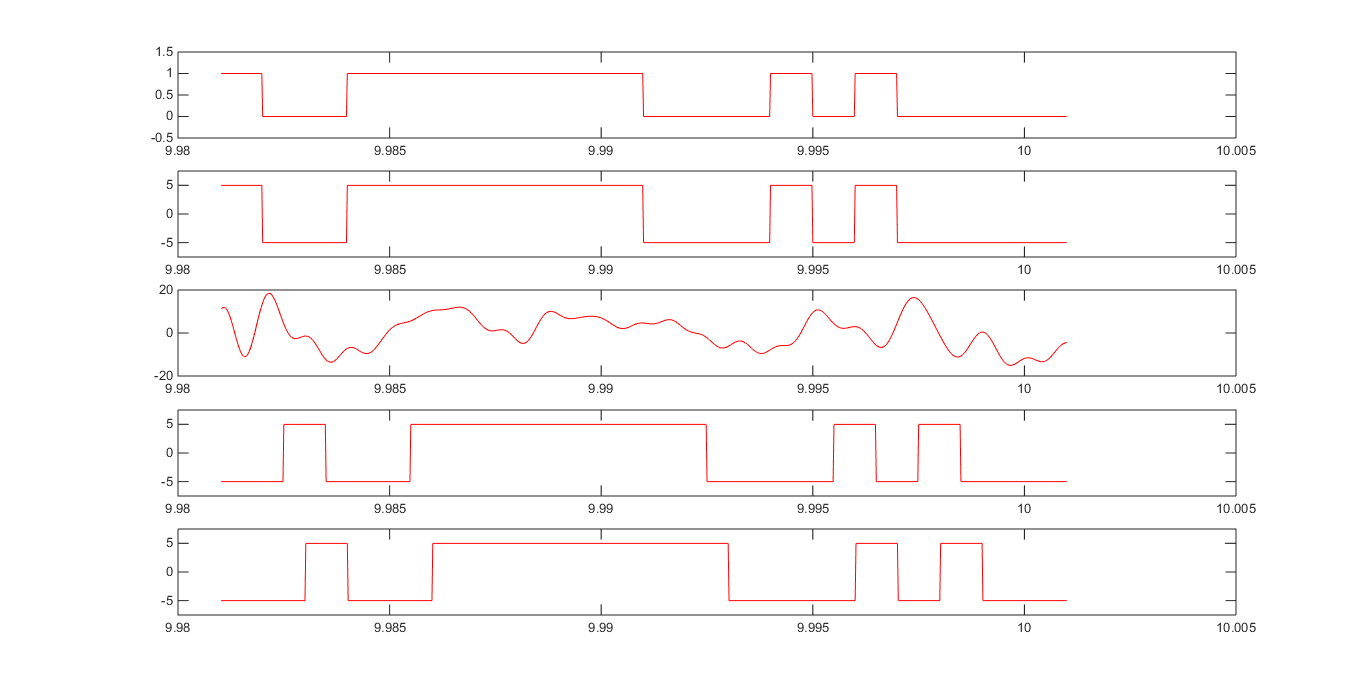
\includegraphics[scale=0.5]{Imagens/Ex2/23}
	\caption{Diversos sinais desde a modula��o � demodula��o.}
	\label{fig_Osci1}
\end{figure}

Por�m pelo fato de ter muitos gr�ficos na mesma imagem, foi optado pela plotagem de \textit{Tx} e \textit{Rx},pela Figura \ref{fig:atraso}, fica evidente o atraso de 3 bits para o dado circuito.

\begin{figure}[H]
	\centering
	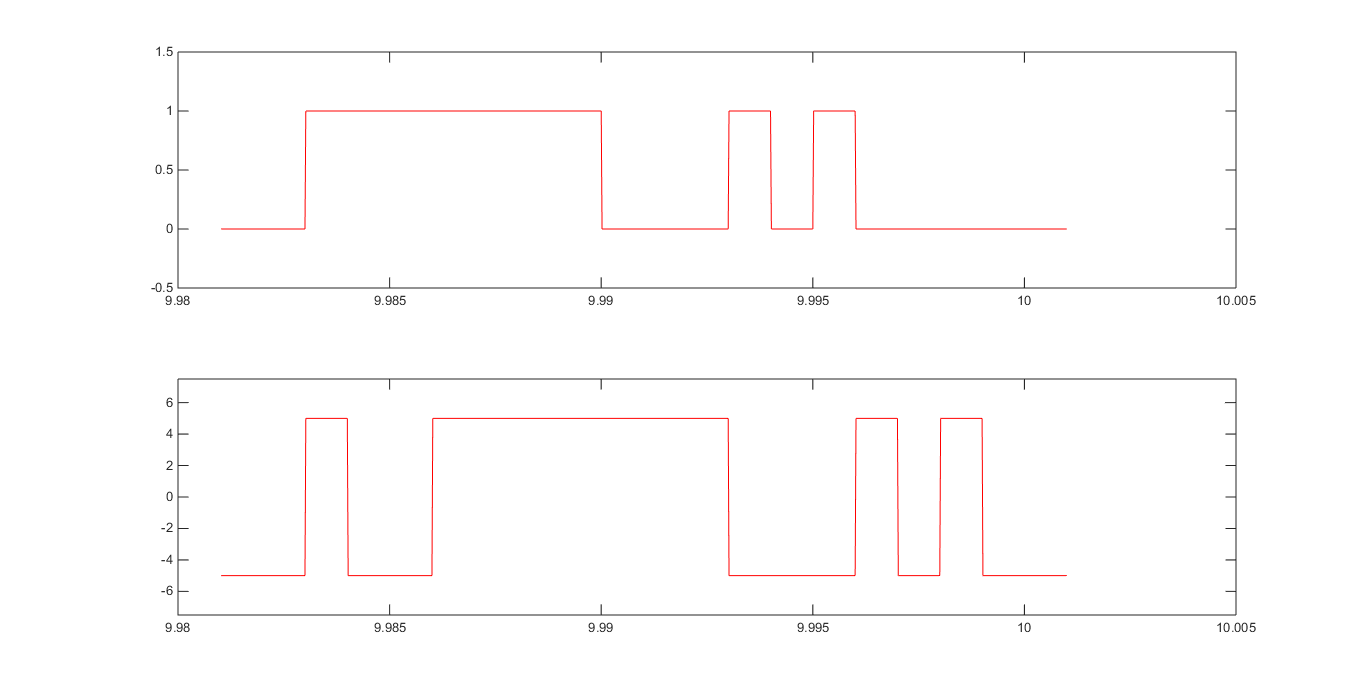
\includegraphics[scale=0.5]{Imagens/Ex2/atraso}
	\caption{Atraso entre Tx e Rx.}
	\label{fig:atraso}
\end{figure}

Com a simula��o devidamente configurada e variando $\sigma^2$ � poss�vel ent�o preencher a Tabela \ref{tab:ber1}.

\begin{center}
	\begin{table}[H]
		\caption{Taxa de erro de bit.}
        \label{tab:ber1}
		\centering\begin{tabular}{c|c|c}
			SNR[dB] & AWGN $\sigma^2$ & BER \\ \hline
			0,97   & 20 & 0,0000 \\
			-3,01  & 50 & 0,0001 \\
			-6,02  & 100 & 0,0051 \\
			-7,78  & 150 & 0,019  \\
			-9,03  & 200 & 0,036  \\
			-10,00 & 250 & 0,052  \\
			-10,33 & 270 & 0,059  \\
			-10,79 & 300 & 0,066  \\
			-13,01 & 500 & 0,11  \\ \hline
		\end{tabular}
	\end{table}
\end{center}

Assim a Figura \ref{fig:BER1}, apresenta o gr�fico da \textit{SNR} por \textit{BER}.

\begin{figure}[H]
	\centering
	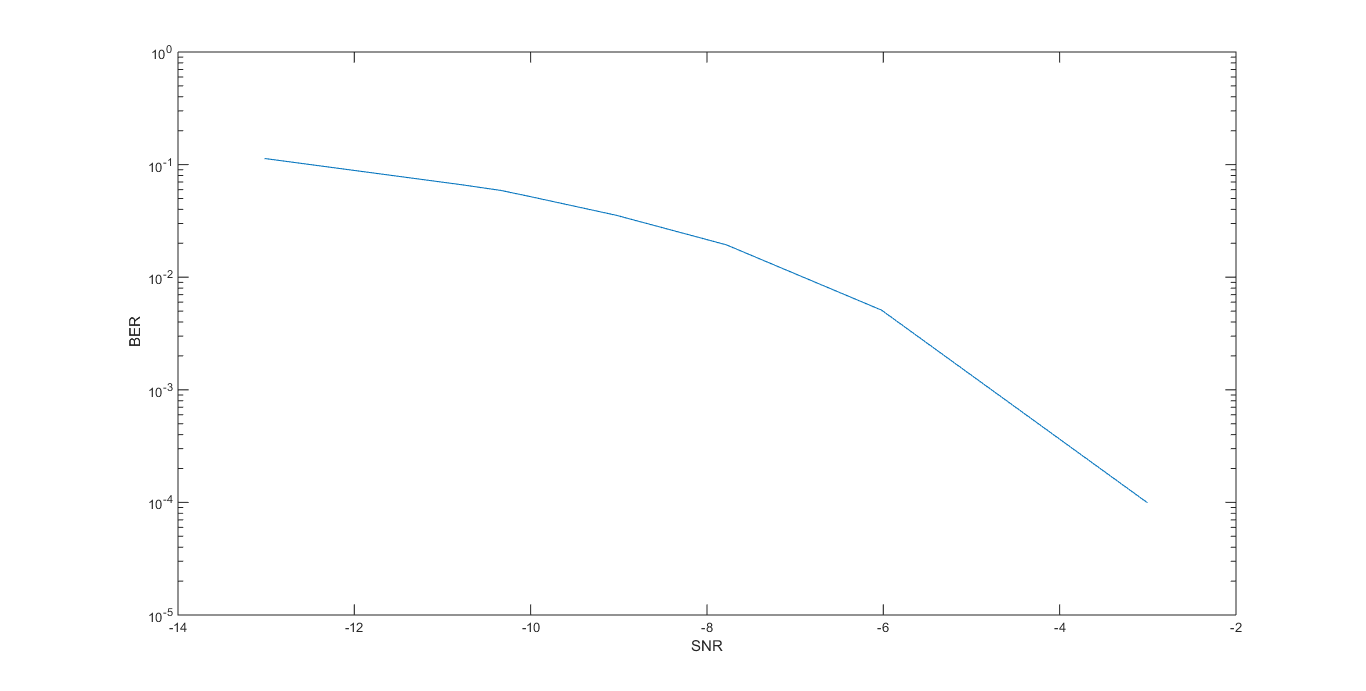
\includegraphics[scale=0.5]{Imagens/Ex2/SNRxBER}
	\caption{Taxa de erro de bit em fun��o da rela��o sinal ru�do.}
	\label{fig:BER1}
\end{figure}

\subsection{PAM sinc}

Com o PAM modulado com sinc da Figura \ref{f2}, foi obtido o gr�fico presente na Figura \ref{fig:sincCent} e \ref{fig:sincMili}.

\begin{figure}[H]
	\centering
	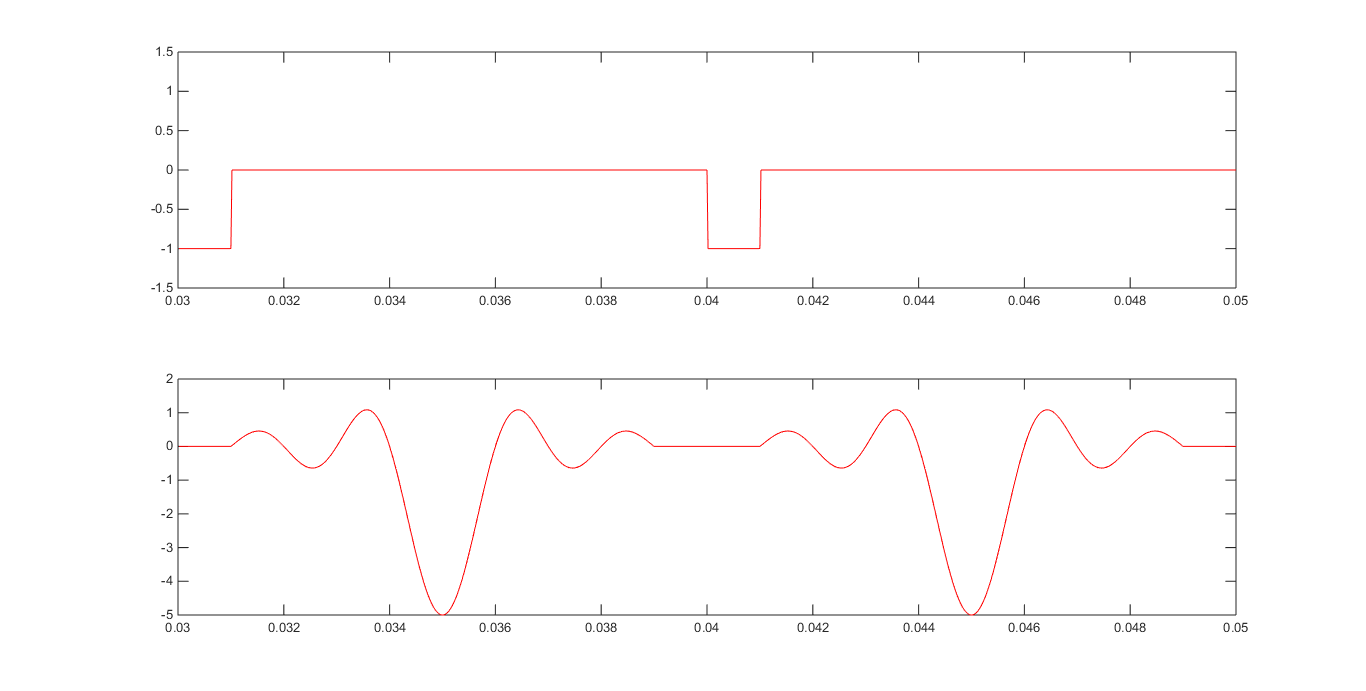
\includegraphics[scale=0.5]{Imagens/Ex3/cent}
	\caption{PAM sinc com taxa de $10^2$.}
	\label{fig:sincCent}
\end{figure}

\begin{figure}[H]
	\centering
	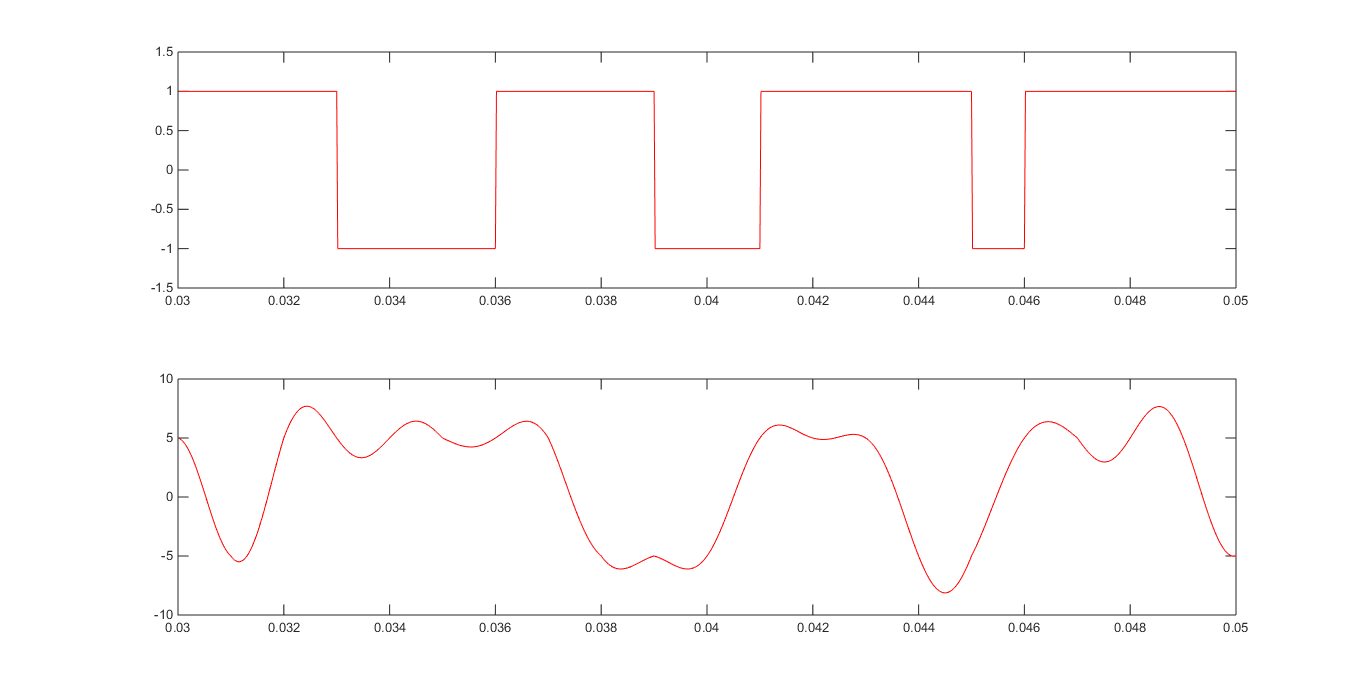
\includegraphics[scale=0.5]{Imagens/Ex3/mili}
	\caption{PAM sinc com taxa de $10^3$.}
	\label{fig:sincMili}
\end{figure}

Para validar a teoria ent�o � colocado um elemento para analisar a \textit{PSD}, densidade espectral de pot�ncia, apresentado na Figura \ref{fig:PSD}.

\begin{figure}[H]
	\centering
	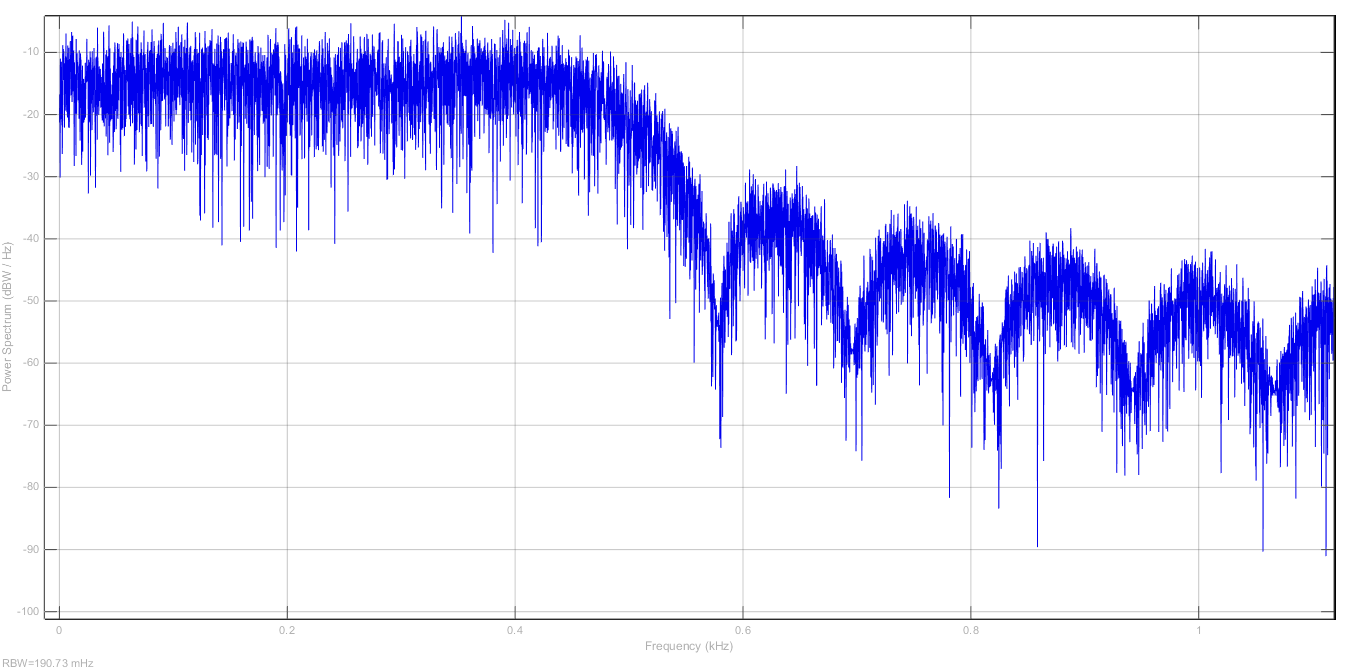
\includegraphics[scale=0.5]{Imagens/Ex4/PSDZOOM}
	\caption{PSD para PAM sinc.}
	\label{fig:PSD}
\end{figure}

Desta forma a frequ�ncia de joelho, � $f_c\approx0,5[kHz]$ o que comprova a teoria pois a banda de um sinal amostrado por uma sinc � metade de um amostrado por uma retangular.

\subsection{PAM sinc por um canal AWGN}

Para o circuito da Figura \ref{f3}, � analisado o atraso a partir da Figura \ref{fig:Rxdemo}.

\begin{figure}[H]
	\centering
	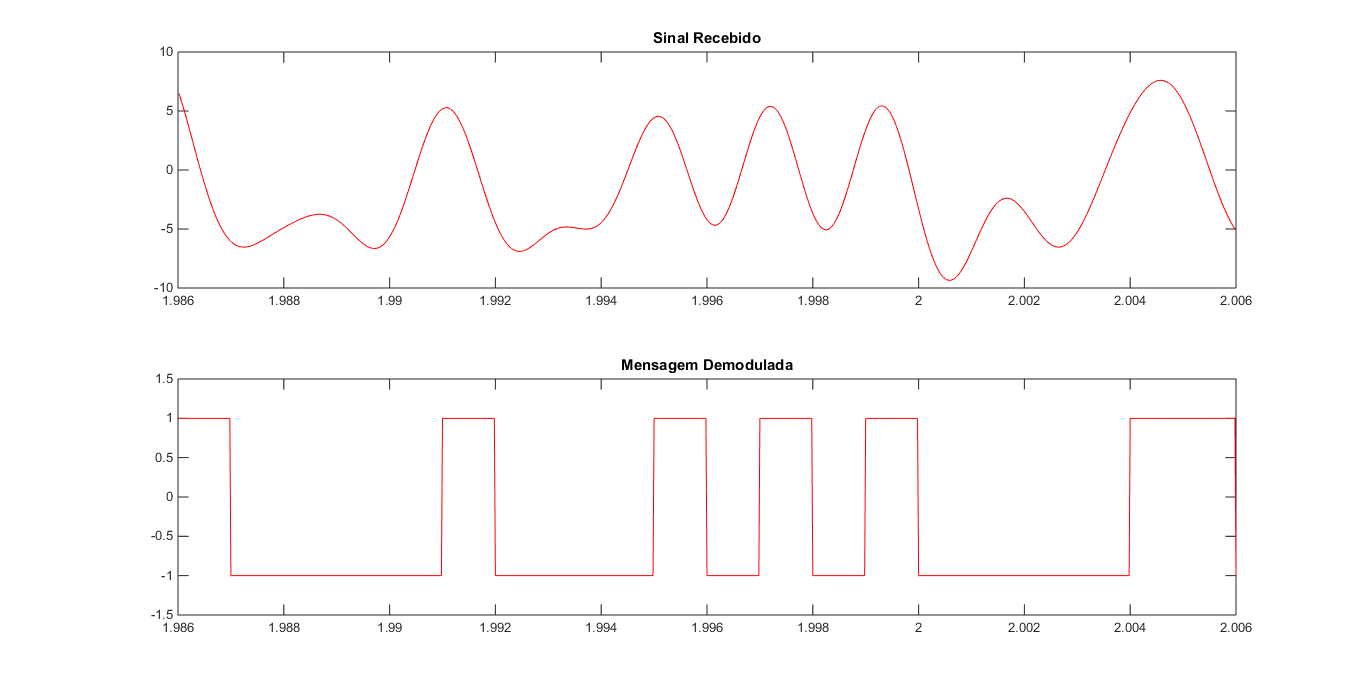
\includegraphics[scale=0.5]{Imagens/Ex5/RxDemo}
	\caption{PAM sinc por um canal AWGN.}
	\label{fig:Rxdemo}
\end{figure}

Assim o atraso de 6 bits fica evidente pela Figura \ref{fig:atraso2}.

\begin{figure}[H]
	\centering
	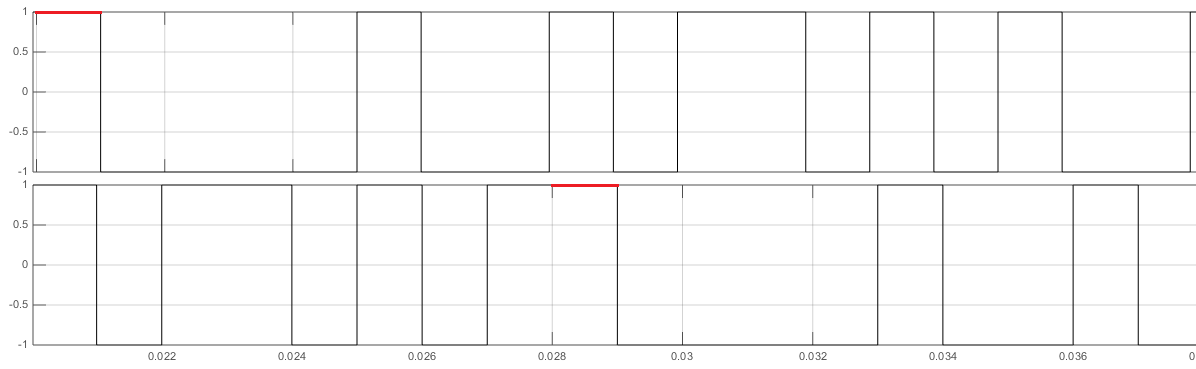
\includegraphics[scale=0.5]{Imagens/Ex5/atraso2}
	\caption{Atraso de 6 bits.}
	\label{fig:atraso2}
\end{figure}

Por fim, para fazer um comparativo e tabelado os valores para diversos $\sigma^2$, de maneira similar a se��o 5.1, obtendo os valores presente na Tabela \ref{tab:ber2}.

\begin{center}
	\begin{table}[H]
		\caption{Taxa de erro de bit.}
		\centering\begin{tabular}{c|c|c}
			SNR[dB] & AWGN $\sigma^2$ & BER \\ \hline
0,85   & 20  & 0      \\
-3,13  & 50  & 0,0004 \\
-6,14  & 100 & 0,004  \\
-7,90  & 150 & 0,011  \\
-9,15  & 200 & 0,023  \\
-10,12 & 250 & 0,030  \\
-10,46 & 270 & 0,037  \\
-10,92 & 300 & 0,046  \\
-13,13 & 500 & 0,091 \\ \hline
		\end{tabular}
		\label{tab:ber2}
	\end{table}
\end{center}

Por fim � realizado um gr�fico comparativo entre o circuito PAM \textit{retangular} e o \textit{sinc}, presente na Figura \ref{fig:BERcomp}.

\begin{figure}[H]
	\centering
	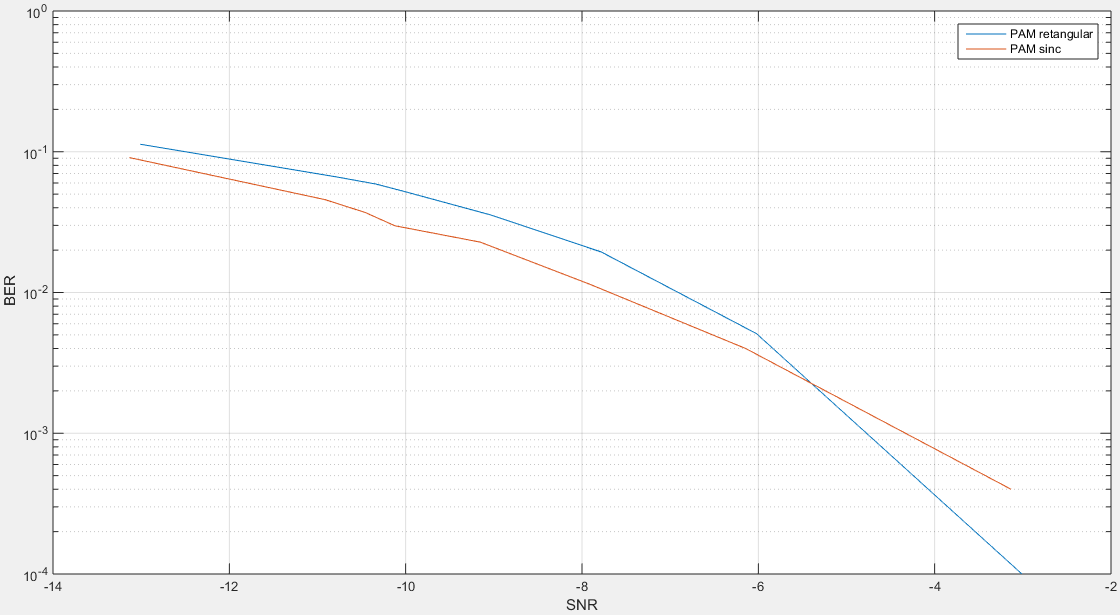
\includegraphics[scale=0.5]{Imagens/Ex5/BERcomp}
	\caption{Comparativo entre os dois tipos de modula��o.}
	\label{fig:BERcomp}
\end{figure}


\newpage

	\section{DISCUSS�ES E CONCLUS�ES}

Como foi constatado nos resultados das simula��es, o fator de m�rito do circuito do mixer � maior que o fator de m�rito do filtro.
Podemos observar tamb�m que, de acordo com a figura \ref{f_saida_up}, o up converter possui uma modula��o AM residual.
Ao analisar a resposta em frequ�ncia tanto do up como do down converter, notamos que o sinal de sa�da possui uma pequena quantidade de energia na primeira harm�nica, por�m, as demais possuem uma energia muito baixa, sendo assim, desprezadas.
Para o caso do mixer com buffer, podemos notar que h� uma n�tida distor��o no sinal do mixer. Essa distor��o gera uma diminui��o da energia da frequ�ncia FI e aumenta a energia das harm�nicas . Vale lembrar que o transistor utilizado n�o � o mesmo do roteiro, sendo assim, o ponto de opera��o do buffer est� deslocado do centro, causando uma interfer�ncia maior na sa�da do circuito.


\pagebreak

\addcontentsline{toc}{section}{REFER�NCIAS}
\nocite{*}
\bibliography{2ELE049.Ref}{}
\bibliographystyle{ieeetr}


\end{document}
%=============================================================================================%
